\documentclass{beamer}
\mode<presentation>
\usetheme{sidebar}
\setbeamertemplate{footline}[page number]

\author{Gijs van der Voort \\ Fabi\"en Tesselaar \\ Richard Torenvliet \\ Tadde\"us Kroes \\ Jayke Meijer}
\title{Local Binary Patterns}

\begin{document}
	
  \section{Wat zijn Local Binary Patterns}
		
  \begin{frame}
    \titlepage
  \end{frame}

  \begin{frame}
    \frametitle{Local Binary Patterns}
    \structure{LBP's als features voor classifier}\\
    \pause
    Aantal voordelen:
    \begin{itemize}
      \item Ongevoelig voor verschillen in belichting. (gray-scale invariant)
      \pause
      \item Simpel algoritme, waardoor voor real-time toepassingen te gebruiken.
    \end{itemize}
  \end{frame}
	
	\section{Hoe werkt het}
  
  \begin{frame}
    \frametitle{Maken van een LBP feature vector}
    \structure{Maken van een LBP}\\
    \begin{itemize}
      \item Kies een pixel
      \pause
      \item Bepaal de buren van de pixel (direct aangrenzende/verder van de pixel vandaan?)
      \pause
      \item Vergelijk de grijswaarde van de eerder gekozen pixel met de grijswaarde van zijn buren
      \pause
      \item Elke vergelijking levert een 1 of 0 op (b.v. groter is 1, kleiner gelijk is 0)
      \pause
      \item Deze binaire waardes samen vormen \'e\'en LBP
    \end{itemize}
  \end{frame}
  
  \begin{frame}
    \frametitle{Maken van een LBP feature vector}
    \structure{Maken van de feature vector}\\
    \begin{itemize}
      \item Verdeel afbeelding in gelijke cellen (b.v. 16x16 pixels per cel)
      \pause
      \item Maak een histogram voor elke cell met de LBP's van die cell
      \pause
      \item Set van histogrammen is de featurevector van het geheel.
      \pause
      \item Featurevector kan gebruikt worden in een SVM.
    \end{itemize}
  \end{frame}
	
	\section{Waar wordt het gebruikt}
  
  \begin{frame}
    \frametitle{Waarvoor wordt het gebruikt}
    Een aantal toepassingen:
    \begin{itemize}
      \item \textbf{Concept Detection}\\
        Herkennen van bepaalde objecten in videobeelden, zoals vliegtuigen, vlaggen etc.
      \item \textbf{Facial Recognition}\\
        Herkennen van gezichten. Ook gebruikt in detecteren van gezichten en herkennen van 
        gezichtsuitdrukkingen.
    \end{itemize}	
  \end{frame}	
	
	\section{Wat doen wij er mee}
  
  \begin{frame}
    \frametitle{Wat doen wij ermee?}
    \structure{License Plate Recognition}\\
    Het lezen van een kenteken.
    \begin{figure}
      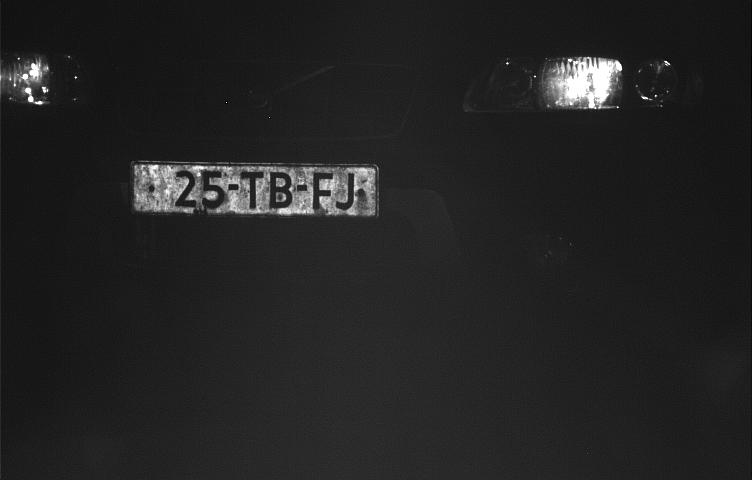
\includegraphics[scale=0.2]{00991_000000.jpg}
    \end{figure}
    Eenvoudige vorm van letters kan goed worden beschreven met een LBP.
  \end{frame}
		
	\section{Conclusie}
	
	\begin{frame}
    \frametitle{Conclusie}
    Vrij simpel algoritme wat zich al heeft bewezen in de werkelijkheid.
  \end{frame}
		
  \begin{frame}
    \frametitle{Bronvermelding}
    \begin{itemize}
      \item \emph{Concept Detection Using Local Binary Patterns and SVM}, Duy-Dinh Le and Shin’ichi Satoh
      \item \emph{Face Description with Local Binary Patterns: Application to Face Recognition}, Timo Ahonen, 	
        Abdenour Hadid and Matti Pietik\"ainen
      \item \emph{Facial expression recognition based on Local Binary Patterns: A comprehensive study}, Caifeng 
        Shan, Shaogang Gong and Peter W. McOwan
      \item \url{http://www.scholarpedia.org/article/Local_Binary_Patterns}
      \item \url{http://en.wikipedia.org/wiki/Local_binary_patterns}
    \end{itemize}
  \end{frame}
	
\end{document}
